%
% domain2.tex -- 
%
% (c) 2019 Prof Dr Andreas Müller, Hochschule Rapperswil
%
\documentclass[tikz,12pt]{standalone}
\usepackage{amsmath}
\usepackage{times}
\usepackage{txfonts}
\usepackage{pgfplots}
\usepackage{csvsimple}
\usetikzlibrary{arrows,intersections,math,calc}
\begin{document}
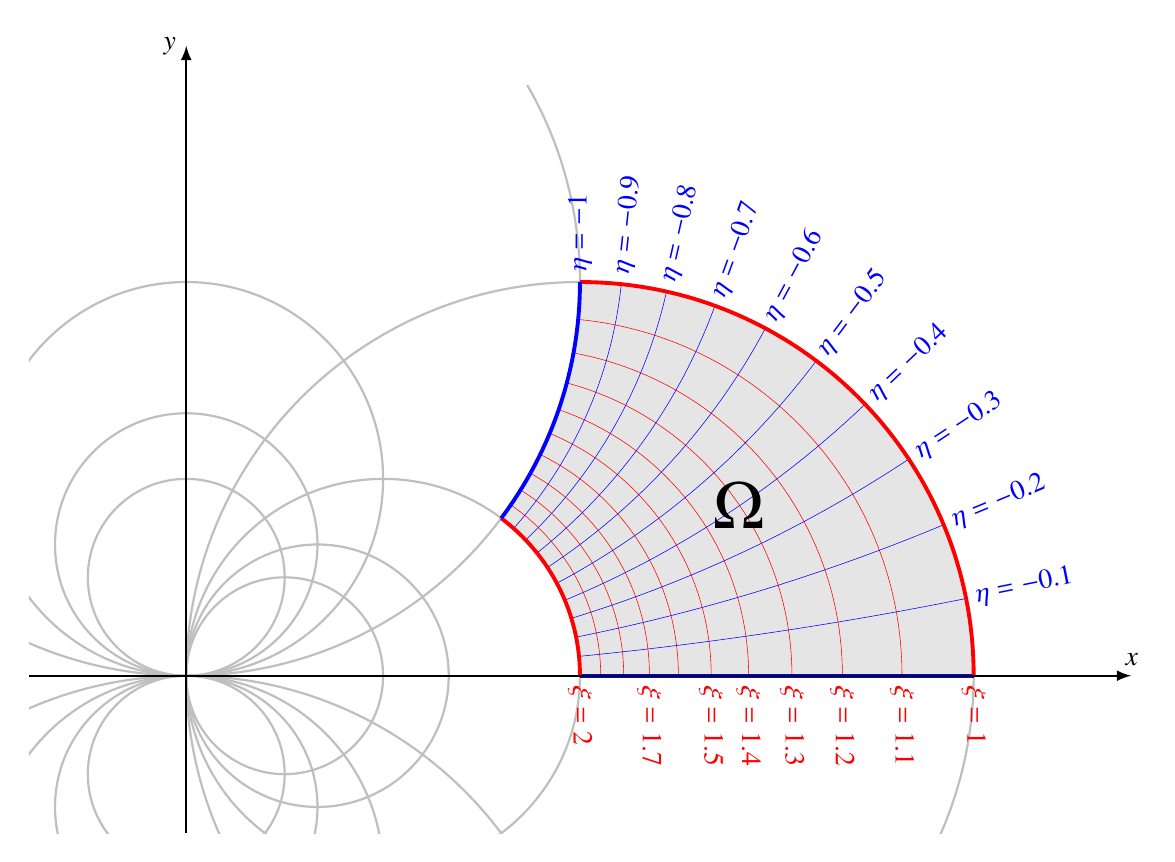
\begin{tikzpicture}[>=latex,thick,scale=10]

\begin{scope}
\clip (-0.2,-0.2) rectangle (1.2,0.75);
\foreach \a in {1,2,3,4}{
	\draw[color=gray!50] ({1/(2*\a)},0) circle[radius={1/(2*\a)}];
}
\foreach \b in {1,2,3,4}{
	\draw[color=gray!50] (0,{1/(2*\b)}) circle[radius={1/(2*\b)}];
	\draw[color=gray!50] (0,{-1/(2*\b)}) circle[radius={1/(2*\b)}];
}
\end{scope}

\pgfmathparse{2/(2*2+1*1)}
\xdef\X{\pgfmathresult}
\pgfmathparse{-1/(2*2+1*1)}
\xdef\Y{\pgfmathresult}
\pgfmathparse{atan(\Y/(\X-0.25))}
\xdef\winkel{\pgfmathresult}

\def\punkt#1#2{
	({#1/((#1)*(#1)+(#2)*(#2))},{-(#2)/((#1)*(#1)+(#2)*(#2))})
}

%\definecolor{darkgreen}{rgb}{0,0.6,0}
%	\draw[color=darkgreen] (0.5,0)
%		-- (1,0) arc (0:90:0.5) 
%		-- (0.5,0.5) arc (0:{-90-\winkel}:0.5)
%		-- (\X,-\Y) arc ({-\winkel}:0:0.25)
%		-- cycle;

\begin{scope}
	\clip (0.5,0)
		-- (1,0) arc (0:90:0.5) 
		-- (0.5,0.5) arc (0:{-90-\winkel}:0.5)
		-- (\X,-\Y) arc ({-\winkel}:0:0.25)
		-- cycle;
	\fill[color=gray!20] (0.5,0) circle[radius=0.5];

	\foreach \a in {1.1,1.2,...,1.9}{
		\draw[color=red,line width=0.2pt]
			({1/(2*\a)},0) circle[radius={1/(2*\a)}];
	}
	\foreach \b in {0.1,0.2,...,0.9}{
		\draw[color=blue,line width=0.2pt]
			(0,{1/(2*\b)}) circle[radius={1/(2*\b)}];
	}
	\fill[color=white] (0.25,0) circle[radius=0.25];
	\fill[color=white] (0,0.5) circle[radius=0.5];
\end{scope}


\draw[color=blue,line width=1.4pt] (0.5,0) -- (1,0);
\draw[color=red,line width=1.4pt] (1,0) arc (0:90:0.5);
\draw[color=red,line width=1.4pt] (0.5,0) arc (0:{-\winkel}:0.25);
\draw[color=blue,line width=1.4pt]
	($(0,0.5)+({-90-\winkel}:0.5)$) arc ({-90-\winkel}:0:0.5);

\draw[->] (-0.2,0) -- (1.2,0) coordinate[label={$x$}];
\draw[->] (0,-0.2) -- (0,0.8) coordinate[label={left:$y$}];


\foreach \a in {0.1,0.2,0.3,0.4,0.5,0.6,0.7,0.8,0.9,1}{
	\pgfmathparse{\a/(\a*\a+1)}
	\xdef\y{\pgfmathresult}
	\pgfmathparse{1/(\a*\a+1)}
	\xdef\x{\pgfmathresult}
	\pgfmathparse{atan(\y/(\x-0.499))}
	\xdef\winkel{\pgfmathresult}
	\node[color=blue] at (\x,\y) [rotate={\winkel},right] {$\eta=-\a$};
}
\foreach \b in {1,1.1,1.2,1.3,1.4,1.5,1.7,2}{
	\node[color=red] at ({1/\b},0) [rotate=-90,right] {$\xi=\b$};
}

%\fill[color=white,opacity=0.7]
%	   \punkt{1.35}{-0.35}
%	-- \punkt{1.25}{-0.35}
%	-- \punkt{1.25}{-0.45}
%	-- \punkt{1.35}{-0.45}
%	-- cycle;
\node at \punkt{1.3}{-0.4} {\Huge $\Omega$};

\end{tikzpicture}
\end{document}

